% \begin{frame}{Lessons \& Philosophy: Adaptation in Life}
%   \centering
%   \begin{columns}
%     \column{0.6\textwidth}
%     \begin{tikzpicture}
%       \begin{axis}[
%         width  = \textwidth,
%         xlabel = Money,
%         ylabel = Happiness,
%         ymin   = 0,
%         ymax   = 1,
%         ytick  = {0, 1},
%         xmin   = 0,
%         xmax   = 1,
%         xtick  = {0, 1},
%         ]

%         \addplot[color=red, mark=x, only marks] coordinates {(0.5, 0.5)};
%         \addplot[color=red, mark=x, only marks] coordinates {(0.4, 0.7)};
%         \addplot[color=red, mark=x, only marks] coordinates {(0.4, 0.6)};

%         \addplot[color=red, mark=x, only marks] coordinates {
%           (0.6, 0.7)
%           (0.5, 0.65)
%           (0.4, 0.55)
%           (0.3, 0.50)
%           (0.2, 0.45)
%           (0.1, 0.20)
%         };
%         \addplot[color=blue, mark=x, only marks] coordinates {
%           (0.83, 0.62)
%           (0.80, 0.59)
%           (0.74, 0.60)
%           (0.63, 0.56)
%           (0.61, 0.36)
%           (0.51, 0.34)
%           (0.50, 0.40)
%           (0.49, 0.41)
%           (0.47, 0.42)
%           (0.46, 0.30)
%           (0.44, 0.25)
%           (0.24, 0.20)
%           (0.10, 0.10)
%         };
%       \end{axis}
%     \end{tikzpicture}

%     \column{0.4\textwidth}
%     \footnotesize

%     Markets/Shops
%     \begin{itemize}
%     \item Berkeley Bowl
%     \item Monterey Market
%     \item Acme
%     \item The Local Butcher Shop
%     \item Sweet Maria's
%     \item Yaoya-san
%     \item $\ldots$
%     \end{itemize}

%   \end{columns}
% \end{frame}

\begin{frame}{Acknowledgment}
  \vspace{2em}
  \begin{figure}
    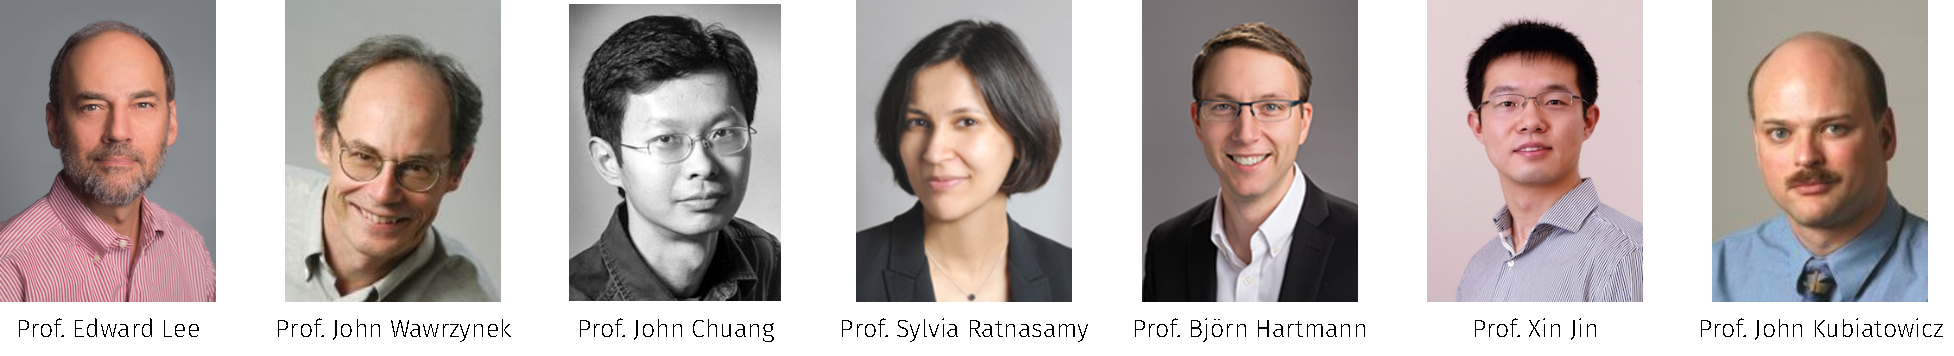
\includegraphics[width=\linewidth]{figures/ack-profs.pdf}
  \end{figure}
  \vspace{-0.5em}
  \pause
  \begin{figure}
    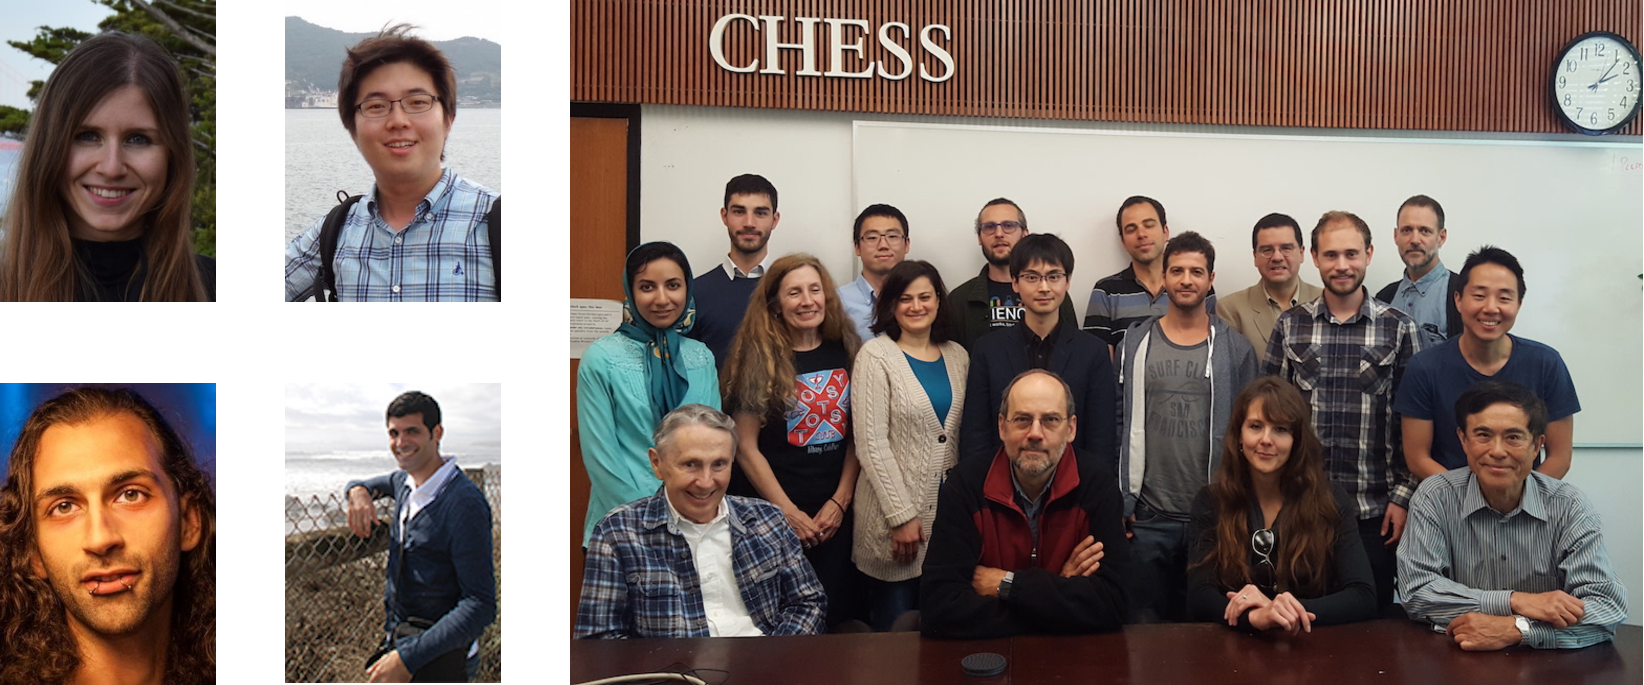
\includegraphics[width=\linewidth]{figures/ack-students.pdf}
  \end{figure}
\end{frame}

\begin{frame}{Acknowledgement}
  \scriptsize \textcolor{ACMRed}{\heartpar{Edward Lee, John Wawrzynek, Syliva
      Ratnasamy, John Chuang, Bj\"orn Hartmann, John Kubiatowicz, Xiaofan Fred
      Jiang, Lin Zhang, David Mellis, Xin Jin, Mary Stewart, Christopher Brooks,
      Eunsuk Kang, Ilge Akkaya, Hokeun Kim, Marten Lohstroh, Matt Weber, Antonio
      Iannopollo, Mehrdad Niknami, Chris Shaver (Yvan Vivid), Michael Zimmer,
      Christos Stergiou, Dai Bui, Ben Lickly, Eleftherios Matsikoudis, Joseph
      Ng, Chadlia Jerad Ep Ben Haj Hmida, Moez Ben Haj Hmida, Maryam Bagheri,
      Victor Nouvellet, Ankush Desai, Nitesh Mor, Yu-Hsiang Sean Chen, Claire
      Tuna, Achal Dave, Jack Kolb, Eric Allman, Roy Wang, Bill N. Schilit, Jin
      Liang, Chao Mei, Kaifei Chen, Qifan Pu, Xiang Gao, Peihan Miao, Zhuo Chen,
      Yuting Wei, Chaoran Guo, Qian Zhong, Tianshi Wang, Meng Wei, Limin Chen}}
\end{frame}

\begin{frame}[standout]
  \begin{columns}
    \column{0.5\textwidth}
    \centering
    1N73LL1G3NC3 \\
    15 7H3 \\
    4B1L17Y \\
    70 4D4P7 70 \\
    CH4NG3

    \pause
    \column{0.5\textwidth}
    \begin{figure}
      \centering
      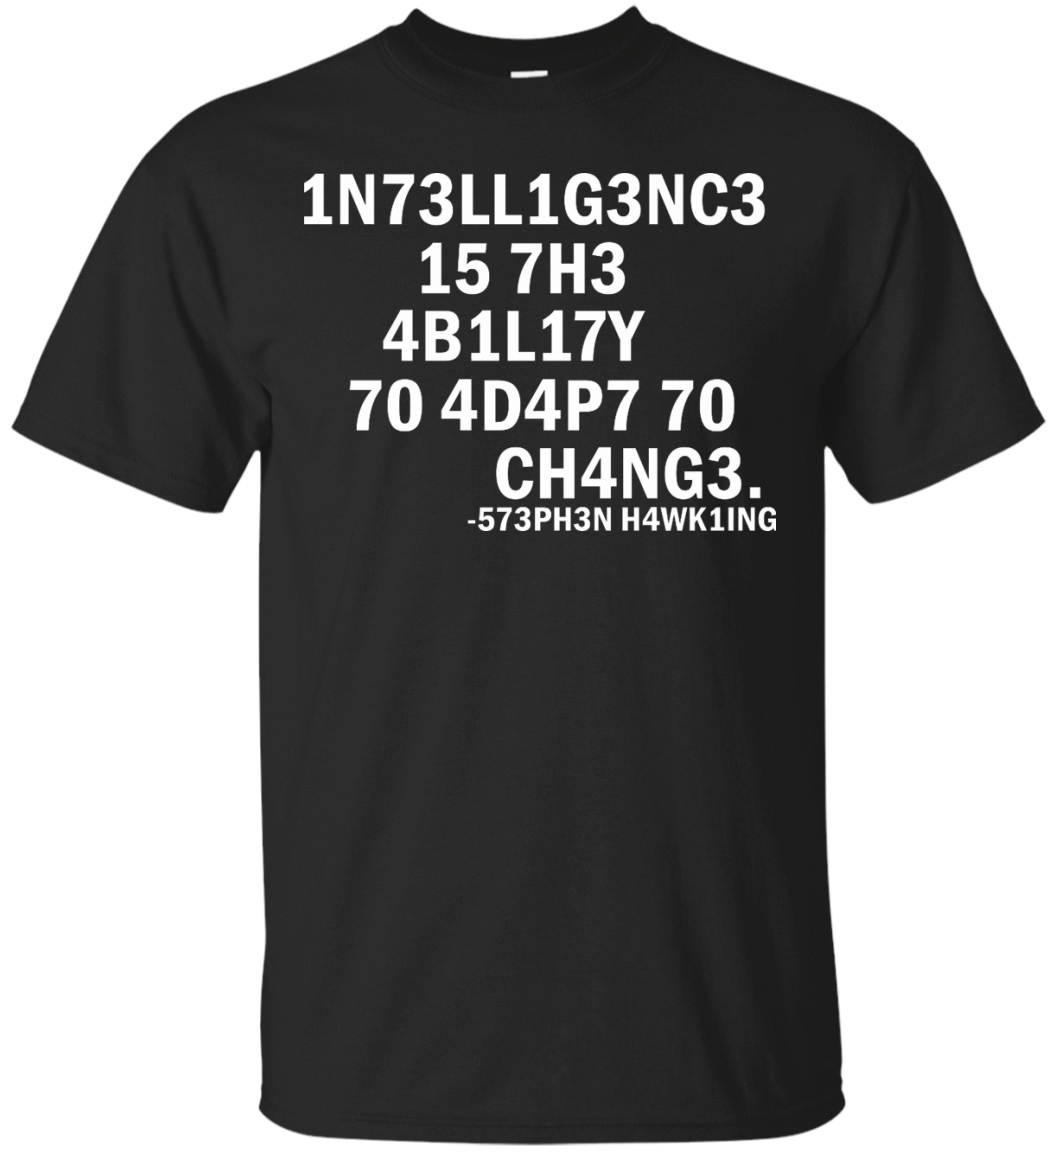
\includegraphics[height=\textwidth]{figures/shirt.png}
      \caption{\color{white} Image Source: \href{https://www.0stees.com/products/intelligence-is-the-ability-to-adapt-to-change-shirt-hoodie-tank?variant=40350207242}{0stees.com}}
    \end{figure}
  \end{columns}
\end{frame}

\begin{frame}
  Google Network Infrastructure

  \begin{figure}
    \centering
    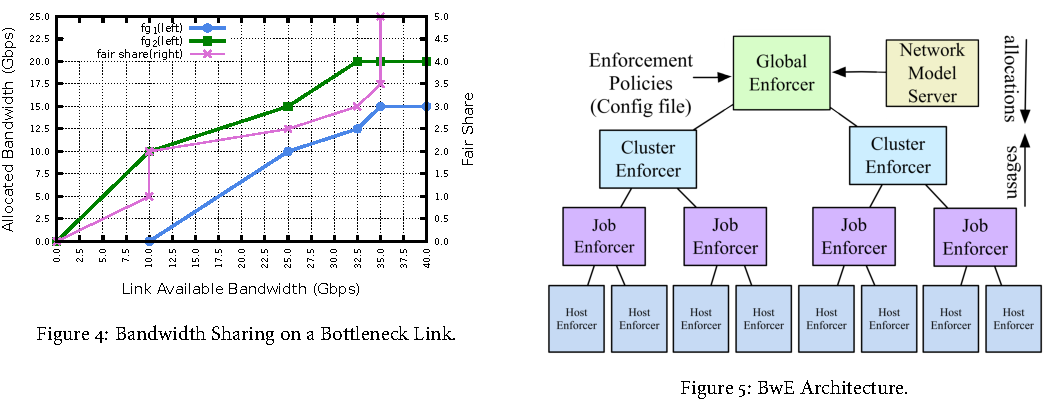
\includegraphics[width=\textwidth]{figures/bwe.pdf}
    \caption{BwE: Flexible, Hierarchical Bandwidth Allocation for WAN
      Distributed Computing~\cite{kumar2015bwe}}
  \end{figure}

  \pause

  Move from Lagrangian to Eulerian (ask Edward if you don't know what these
  words refer to).

\end{frame}

% \begin{frame}
%   Twitter, Pub/Sub, Stream Processing
% \end{frame}

%%% Local Variables:
%%% mode: latex
%%% TeX-master: "talk"
%%% TeX-engine: xetex
%%% End:
